\setcounter{chapter}{16}
\exam{Teste 1 2017/18}
\question{Pergunta 1}
\begin{alignat*}{1}
	f(x) &= (x-3.6)+\cos^3(x+1.2)\\
	f'(x) &= 1-3\cos^2(x+1.2)\sin(x+1.2)
\end{alignat*}
\begin{equation*}
	g(x)
	= x-\frac{f(x)}{f'(x)}
	= \frac{-\cos^2(x+1.2)[3x\sin(x+1.2)+\cos(x+1.2)]+3.6}{1-3\cos^2(x+1.2)\sin(x+1.2)}
\end{equation*}
Se definirmos
\begin{gather*}
	x' = x+1.2\\
	c = \cos(x')\\
	s = \sin(x')\\
	d = c^2
\end{gather*}
ficamos com
\begin{equation*}
	g(x)
	= \frac{-d(3xs+c)+3.6}{1-3ds}
\end{equation*}
\lstinputlisting[language=C++, caption=Código-fonte 2017T1-1 (C++)]{01.cpp}
\begin{center}
\begin{tabular}{ p{73mm} p{0mm} p{73mm} }
	\lstinputlisting[caption=Input 2017T1-1]{01.in} & &
	\lstinputlisting[caption=Output 2017T1-1]{01.out}
\end{tabular}
\end{center}

\question{Pergunta 2}
Utilizaria a fórmula \ref{itm:2017T1-2a}, uma vez que:
\begin{enumerate}[label=\textbf{(\alph*)}]
	\item \label{itm:2017T1-2a} Tem concavidade voltada para cima e é crescente em $x > 0$, pelo que se $x_n > \xi_x$ a tangente nesse ponto interseta o eixo das abcissas em $x_{n+1} >\xi_x $ mais próxima de $\xi_x$ do que $x_n$. Agora, basta usar um guess $>= \xi_x$; se $x>1$, o guess pode ser $R$, se $x\leq1$ o guess pode ser $1$.
	\begin{center} 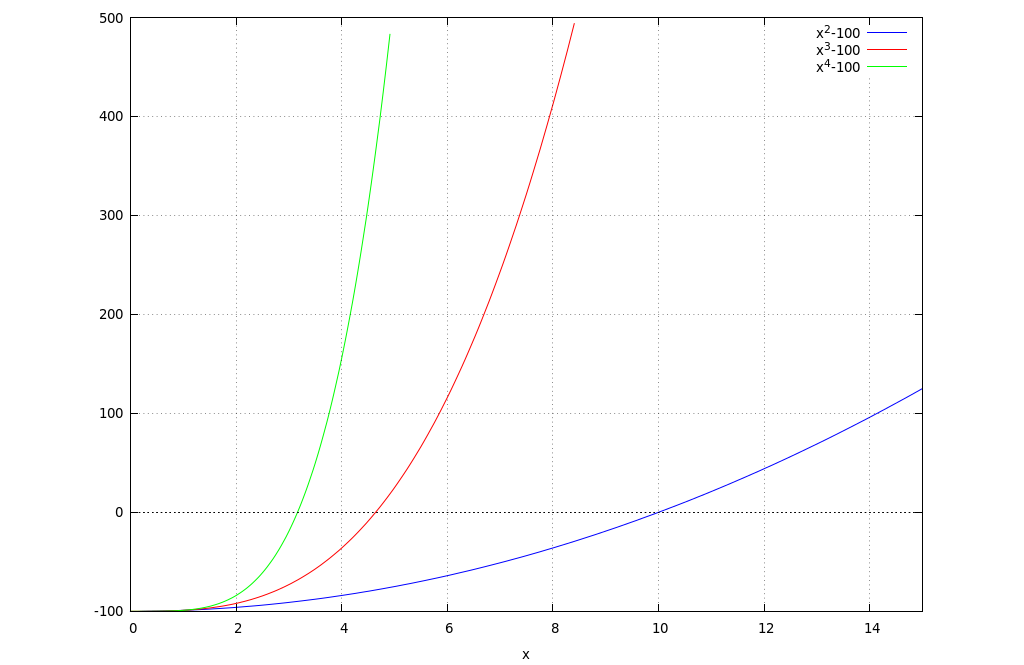
\includegraphics[height=60mm,keepaspectratio]{plot2017T1-2a} \end{center}
	\item \label{itm:2017T1-2b} Tem concavidade voltada para baixo e é crescente em $x > 0$, pelo que teria que se verificar $0 < x_n < \xi_x$ para que a tangente nesse ponto intersete o eixo das abcissas em $x_{n+1}$ que verifica $0<x_{n+1}<\xi_x$ e que está mais próximo de $\xi_x$ do que $x_n$; mas o guess também não pode ser demasiado próximo de $0$, uma vez que o declive de $f(x)=1-R/x^m$ é muito elevado na proximidade de $0$, o que significa que a convergência é lenta.
	\begin{center} 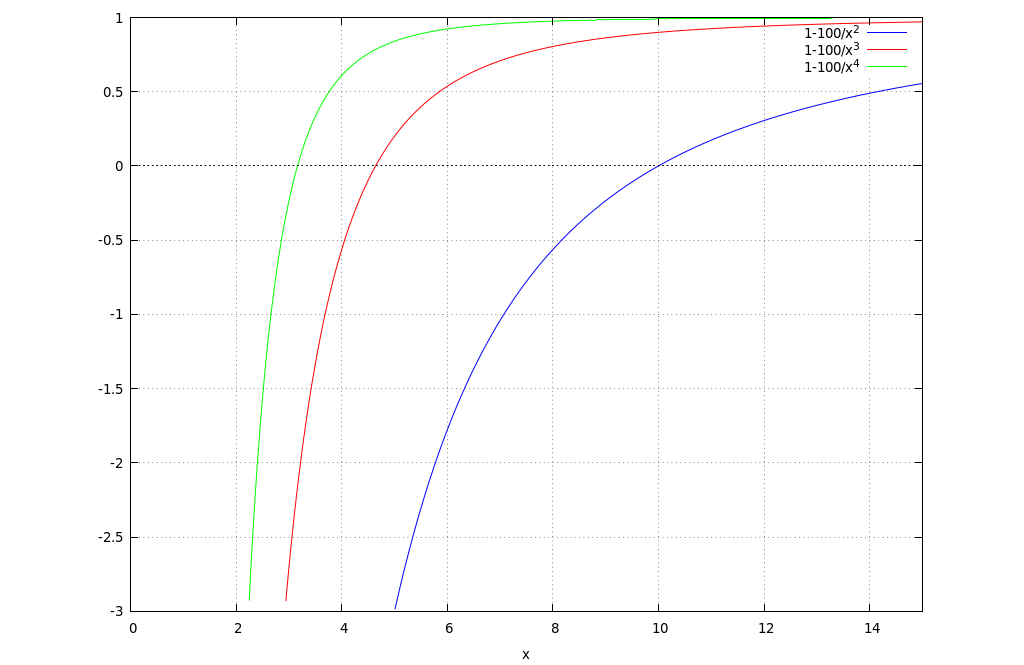
\includegraphics[height=60mm,keepaspectratio]{plot2017T1-2b} \end{center}
\end{enumerate}
Em ambos os exemplos, são utilizados os parâmetros $R=100$ e $m=2,3,4$.\\
Em suma, é mais fácil determinar um guess para \ref{itm:2017T1-2a} do que para \ref{itm:2017T1-2b}, além de \ref{itm:2017T1-2a} convergir mais depressa do que \ref{itm:2017T1-2b}.

\lstinputlisting[language=Python, caption=Código-fonte 2017T1-2 (Python3)]{02.py}
\begin{center}
\begin{tabular}{ p{70mm} p{0mm} p{76mm} }
	\lstinputlisting[caption=Input 2017T1-2]{02.in} & &
	\lstinputlisting[caption=Output 2016T1-2]{02.out}
\end{tabular}
\end{center}
\question{Pergunta 5}
Com truncagem.
\begin{center}
\begin{tabular}{>{\rowmac}c||>{\rowmac}c|>{\rowmac}c|>{\rowmac}c|>{\rowmac}c||>{\rowmac}c|>{\rowmac}c||>{\rowmac}l>{\rowmac}l<{\clearrow}}
op                &$\pm{}$&\multicolumn{3}{c||}{mantissa}&$\pm{}$&exp& \multicolumn{2}{c}{comentários}\\ \hline \hline
                  & + & 1 & 3 & 3 & + & 0 & $x=2/15              $ & $\SI{+0.133e+0}{}$\\
$\ast            $& + & 1 & 3 & 3 & + & 0 & $x                   $ & $\SI{+0.133e+0}{}$\\ \hline
                  & + & 1 & 7 & 6 & - & 1 & $x^2=0.017689        $ & $\SI{+0.176e-1}{}$\\
$\ast            $& + & 1 & 3 & 3 & + & 0 & $x                   $ & $\SI{+0.133e+0}{}$\\ \hline
                  & + & 2 & 3 & 4 & - & 2 & $x^3=0.0023408       $ & $\SI{+0.234e-2}{}$\\
\setrow{\bfseries}& - & 2 & 0 & 0 & + & 1 & $-2                  $ & $\SI{-0.200e+1}{}$\\
                  & + & 1 & 3 & 3 & + & 0 & $x                   $ & $\SI{+0.133e+0}{}$\\
$\ast            $& + & 4 & 0 & 0 & + & 1 & $4                   $ & $\SI{+0.400e+1}{}$\\ \hline
\setrow{\bfseries}& + & 5 & 3 & 2 & + & 0 & $4x=0.532            $ & $\SI{+0.532e+0}{}$\\
                  & + & 1 & 7 & 6 & - & 1 & $x^2                 $ & $\SI{+0.176e-1}{}$\\
$\ast            $& - & 3 & 0 & 0 & + & 1 & $-3                  $ & $\SI{-0.300e+1}{}$\\ \hline
\setrow{\bfseries}& - & 5 & 2 & 8 & - & 1 & $-3x^2=-0.0528       $ & $\SI{-0.528e-1}{}$\\
                  & + & 2 & 3 & 4 & - & 2 & $x^3                 $ & $\SI{+0.234e-2}{}$\\
$\ast            $& + & 5 & 0 & 0 & + & 1 & $5                   $ & $\SI{+0.500e+1}{}$\\ \hline
\setrow{\bfseries}& + & 1 & 1 & 7 & - & 1 & $5x^3=0.0117         $ & $\SI{+0.117e-1}{}$
\end{tabular}
\end{center}
Efetuando as operações pela ordem
\begin{equation*}
	((5x^3-3x^2)+4x)-2
\end{equation*}
\begin{center}
\begin{tabular}{>{\rowmac}c||>{\rowmac}c|>{\rowmac}c|>{\rowmac}c|>{\rowmac}c||>{\rowmac}c|>{\rowmac}c||>{\rowmac}l>{\rowmac}l<{\clearrow}}
op    &$\pm{}$&\multicolumn{3}{c||}{mantissa}&$\pm{}$&exp& \multicolumn{2}{c}{comentários}\\ \hline \hline
      & + & 1 & 1 & 7 & - & 1 & $5x^3                $ & $\SI{+0.117e-1}{}$\\
+     & - & 5 & 2 & 8 & - & 1 & $-3x^2               $ & $\SI{-0.528e-1}{}$\\ \hline
      & - & 4 & 1 & 1 & - & 1 & $5x^3-3x^2=-0.0411   $ & $\SI{-0.411e-1}{}$\\
      & - & 0 & 4 & 1 & + & 0 & $5x^3-3x^2           $ & $\SI{-0.041e+0}{}$\\
+     & + & 5 & 3 & 2 & + & 0 & $4x                  $ & $\SI{+0.532e+0}{}$\\ \hline
      & + & 4 & 9 & 1 & + & 0 & $5x^3-3x^2+4x=0.491  $ & $\SI{+0.491e+0}{}$\\
      & + & 0 & 4 & 9 & + & 1 & $5x^3-3x^2+4x        $ & $\SI{+0.049e+1}{}$\\
+     & - & 2 & 0 & 0 & + & 1 & $-2                  $ & $\SI{-0.200e+1}{}$\\ \hline
      & - & 1 & 5 & 1 & + & 1 & $5x^3-3x^2+4x-2=-1.51$ & $\SI{-0.151e+1}{}$
\end{tabular}
\end{center}
Efetuando agora as operações pela ordem
\begin{equation*}
	5x^3-(3x^2+(4x-2))
\end{equation*}
\begin{center}
\begin{tabular}{>{\rowmac}c||>{\rowmac}c|>{\rowmac}c|>{\rowmac}c|>{\rowmac}c||>{\rowmac}c|>{\rowmac}c||>{\rowmac}l>{\rowmac}l<{\clearrow}}
op    &$\pm{}$&\multicolumn{3}{c||}{mantissa}&$\pm{}$&exp& \multicolumn{2}{c}{comentários}\\ \hline \hline
      & - & 2 & 0 & 0 & + & 1 & $-2                  $ & $\SI{-0.200e+1}{}$\\
+     & + & 5 & 3 & 2 & + & 0 & $4x                  $ & $\SI{+0.532e+0}{}$\\
+     & + & 0 & 5 & 3 & + & 1 & $4x                  $ & $\SI{+0.053e+1}{}$\\ \hline
      & - & 1 & 4 & 7 & + & 1 & $4x-2=-1.47          $ & $\SI{-0.147e+1}{}$\\
+     & - & 5 & 2 & 8 & - & 1 & $-3x^2               $ & $\SI{-0.528e-1}{}$\\
+     & - & 0 & 0 & 5 & + & 1 & $-3x^2               $ & $\SI{-0.005e+1}{}$\\ \hline
      & - & 1 & 5 & 2 & + & 1 & $-3x^2+4x-2=-1.52    $ & $\SI{-0.152e+1}{}$\\
+     & + & 1 & 1 & 7 & - & 1 & $5x^3                $ & $\SI{+0.117e-1}{}$\\
+     & + & 0 & 0 & 1 & + & 1 & $5x^3                $ & $\SI{+0.001e+1}{}$\\ \hline
      & - & 1 & 5 & 1 & + & 1 & $5x^3-3x^2+4x-2=-1.51$ & $\SI{-0.151e+1}{}$
\end{tabular}
\end{center}
Utilizando arredondamento ou truncagem, por ambas as ordens de operações, o resultado é sempre $-1.51$. Ou seja, não foi possível encontrar formas que dessem resultados diferentes.
